% BRED

\section{Introduction}

One of the central cellular processes underlying development is transcriptional regulation. During development, changes in transcription factor activity induce chromatin modifications, chromatin remodelling and ultimately a differential recruitment of the basal transcriptional machinery\cite{coulon_eukaryotictranscriptionaldynamics_2013}. Modelling the dynamics of gene regulation is therefore essential to better understand why a cellular dynamic processes progresses through several steps, and what goes wrong in the case of disease.

The dynamics of gene regulation has classically been studied using time series data\cite{bar-joseph_studyingmodellingdynamic_2012}. When dynamic processes progress asynchronously, such as in hematopoiesis, time series data are usually obtained by sorting different transition states and assessing bulk gene expression and transcription factor binding within the population\cite{novershtern_denselyinterconnectedtranscriptional_2011, may_dynamicanalysisgene_2013, jojic_identificationtranscriptionalregulators_2013, goode_dynamicgeneregulatory_2016}. Alternatively, time series data can also be generated by synchronizing the dynamic process between cells. However, issues with time-resolution, heterogeneity and good in vivo synchronization models can often limit the predictive power of the dynamic models of gene regulation which can be constructed\cite{bar-joseph_studyingmodellingdynamic_2012}.

One of the main advantages of single-cell transcriptomics is the ability to quantify the exact cellular state of thousands of cells per experiment. The intercellular heterogeneity caused by naturally occurring biological stochasticity \cite{padovan-merhar_usingvariabilitygene_2013} can be exploited to predict regulatory interactions between transcription factors (TFs) and their target genes. The computational tools that infer gene regulatory networks (GRNs) from omics datasets are called network inference (NI) methods.
% TODO: talk about bulk NI

Several studies have highlighted how some regulatory interactions can be very dynamic while others show evidence of being static during consecutive developmental stages\cite{moignard_characterizationtranscriptionalnetworks_2013, pina_singlecellnetworkanalysis_2015}. 
Since regulatory interactions are context-dependent\cite{papp_genomewideanalysiscontextdependence_2005}, attempting to create an accurate model of those processes by inferring a static regulatory network may have limited relevance.
Case-wise NI methods\footnote{Case-wise NI is sometimes also called sample-specific NI or case-specific NI.} avoid predicting a static GRN and instead infer one GRN per cell (or per sample, for bulk omics data).

In order to compute a case-wise GRN for a single sample, Kuijjer et al.\cite{kuijjer_estimatingsamplespecificregulatory_2019} and Liu et al.\cite{liu_personalizedcharacterizationdiseases_2016} employ similar strategies, namely by computing the difference of computing a static GRN for all the cases, and computing a static GRN for all the cases minus one. Since this procedure needs to be repeated for every case in the dataset, and because NI methods are already amongst the most computationally intensive analyses to perform on omics data, this methodology is not applicable for large omics datasets.
Another case-wise NI method, SCENIC\cite{aibar_scenicsinglecellregulatory_2017} infers case-wise GRNs by first inferring a static GRN using GENIE3\cite{huynh-thu_inferringregulatorynetworks_2010}. GENIE3 is a static NI method which uses Random Forests\cite{breiman_randomforests_2001} feature importance scores to prioritise candidate regulators for a particular target gene. SCENIC then post-processes the static GRN to determine whether an interaction is enriched for particular cases, resulting in a case-wise GRN. 
In short, while several case-wise NI methods thus already exist, their implementation consisted of post-processing a static GRN to arrive at a case-wise GRN. 

In this work, we introduce \texttt{bred}, the first 'true' case-wise NI method. For each interaction in the inferred case-wise GRN, \texttt{bred} predicts both the regulatory strength and its effect. 
The case-wise GRNs -- or 'case-wise regulomes' -- can be analysed analogously to transcriptomics data; for example by clustering samples, inferring trajectories, or finding differentially activated regions.
We demonstrate \texttt{bred} by applying it to a single-cell dataset of 22'122 hematopoietic cells from the Tabula Muris project\cite{schaum_singlecelltranscriptomics20_2018}, and to a collection of 14'963 bulk omics samples from The Cancer Genome Atlas project\cite{weinstein_cancergenomeatlas_2013}.


\section{Results}


\subsection{Hematopoietic cells from Tabula Muris}
From the Tabula Muris\cite{schaum_singlecelltranscriptomics20_2018} project, we selected all cells involved in some part of the hematopoietic lineage tree. We computed case-wise GRNs between 22'122 remaining single cells, for the 2000 most variable target genes and a subset of transcription factors as regulators.

To summarise the similarity in GRNs across cases, we first visualise a dimensionality reduction of the case-wise GRNs, where every dot represents a single GRN (Figure~\ref{fig:tabmur}A). The dimensionality reduction was computed by applying Fruchterman-Reingold\cite{fruchterman_graphdrawingforcedirected_1991} on the $k$-nearest-neighbour ($k$NN) graph of the case-wise GRN vectors. On the same $k$NN graph, the cells were clustered using the Louvain\cite{blondel_fastunfoldingcommunities_2008} clustering algorithm, and the clusters were labelled using prior information from Tabula Muris.
For each cluster, we retained the 50 interactions with the highest mean importance scores (Figure~\ref{fig:tabmur}B). In the visualisation, each node represents a gene, each edge an interaction, and the colour represents which cluster this interaction belongs to.

For the most part, clusters that are proximate in the dimensionality reduction (Figure~\ref{fig:tabmur}A) are also closely connected in the GRN network view (Figure~\ref{fig:tabmur}B). Notably, interactions from the different B cell clusters are almost not connected amongst each-other, while in the dimensionality reduction they re very proximate. Retaining more edges could result in the different B cells being connected in the GRN network view.

At the centre of the network lie many strongly connected interactions which are not specific for any particular cluster, but instead are common to almost all of the clusters. These are likely housekeeping genes or genes involved in key hematopoietic processes. 


\begin{figure}[htb!]
	{\raggedright\textbf{A}}
	\begin{center}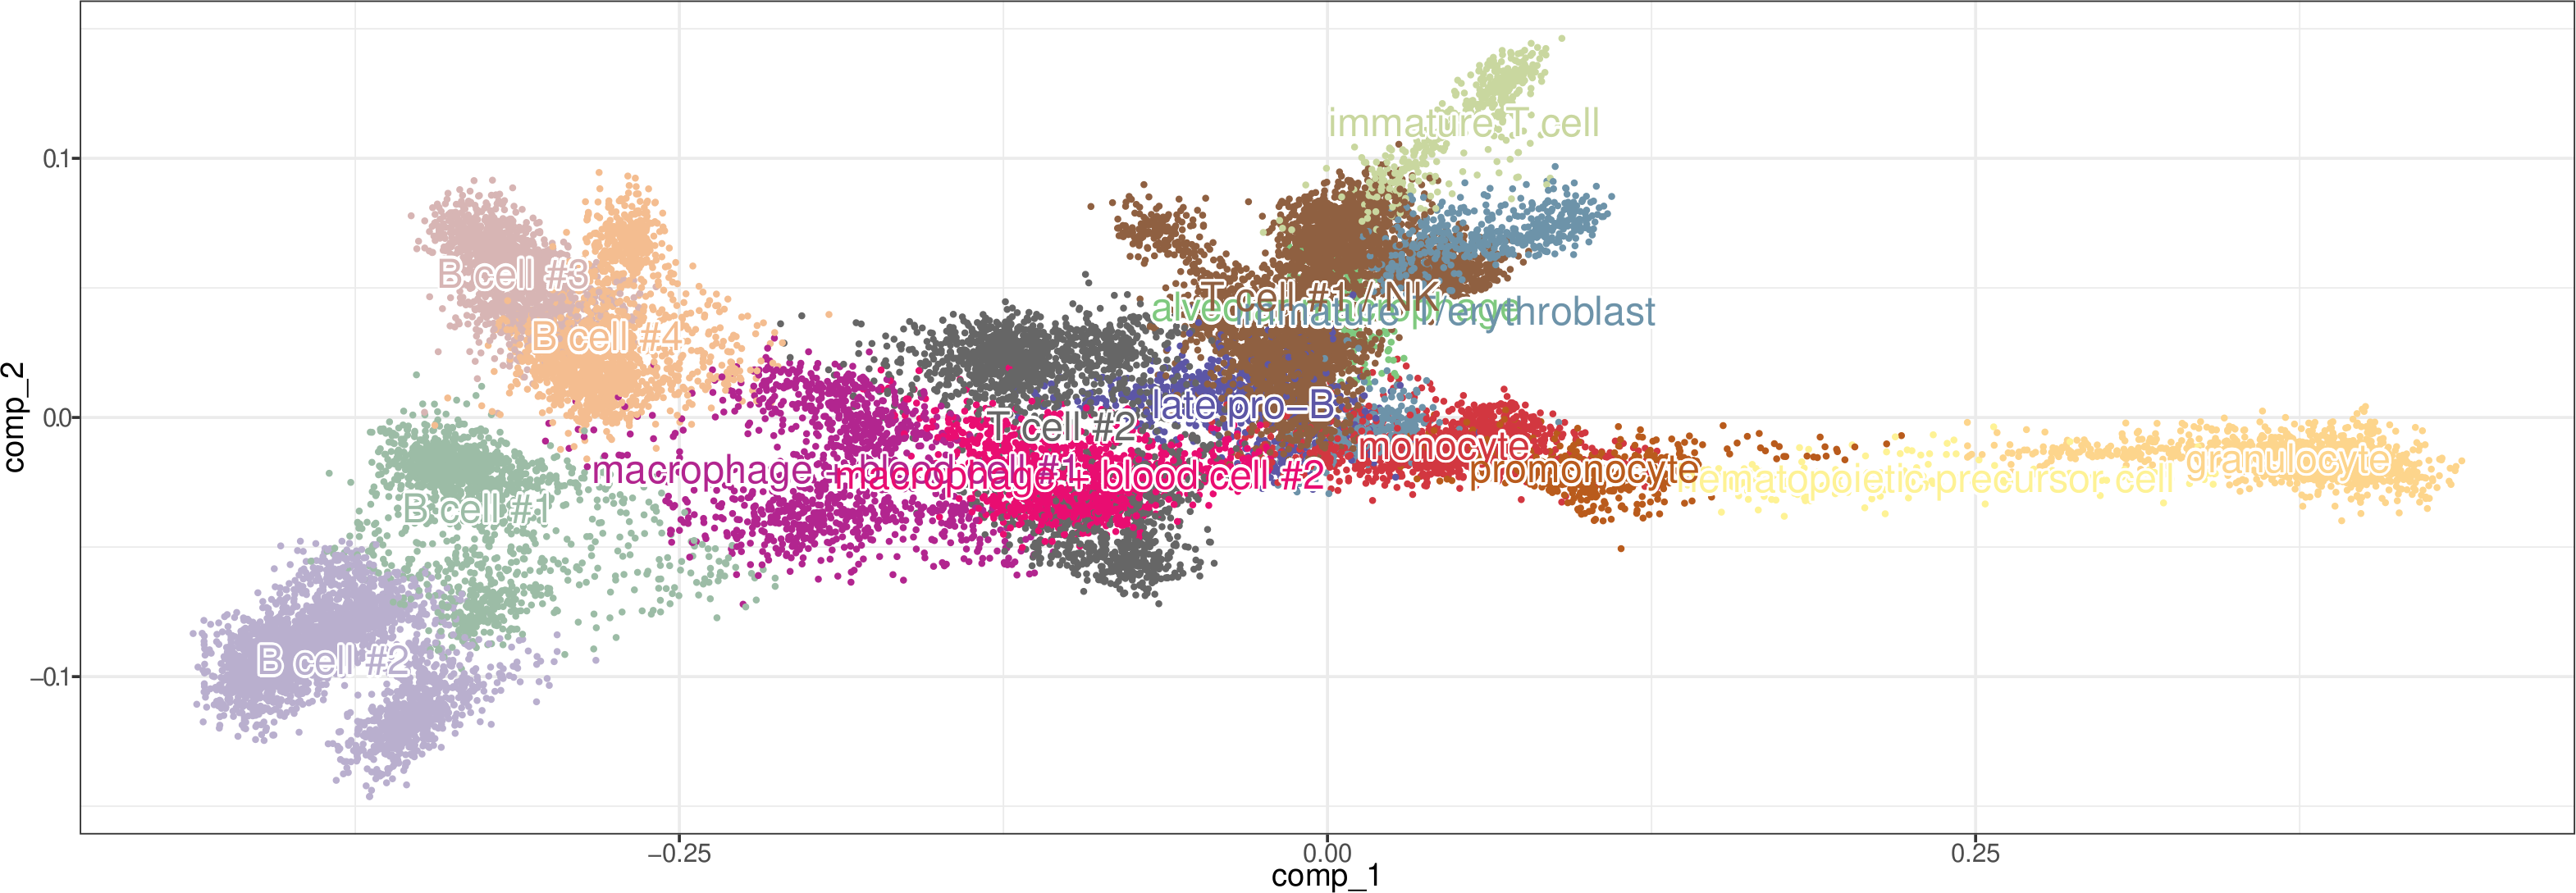
\includegraphics[width=\linewidth]{fig/tabula_muris_hema/plot_fr_cropped.png}\end{center}
	{\raggedright\textbf{B}}
	\begin{center}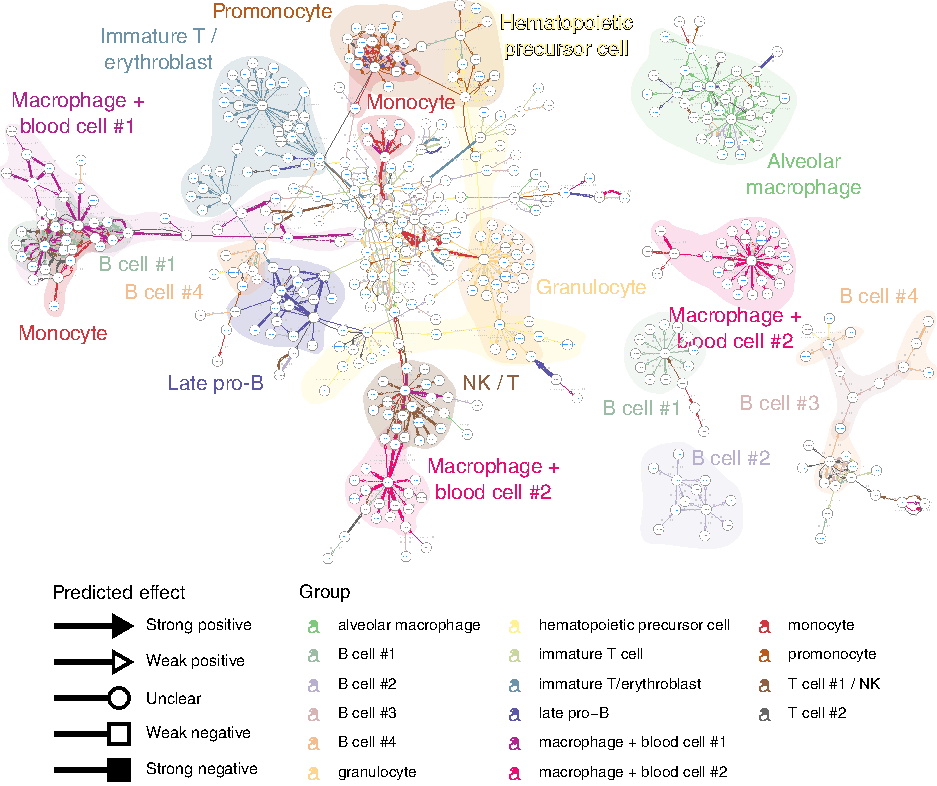
\includegraphics[width=.9\linewidth]{fig/tabula_muris_hema/grouped_interactions.pdf}\end{center}
	\caption{
		\textbf{22'122 case-wise GRNs of hematopoietic cells from the Tabula Muris project.}
		\textbf{A:} Each dot in this dimensionality reduction corresponds to the GRN of a single cell. The dimensionality of the cell-specific regulome matix was reduced using Fruchterman-Reingold and were clustered using Louvain clsutering, after which the clusters were relabelled using the meta information from Tabula Muris.
		\textbf{B:} Per cluster, the 50 interactions with the highest mean importance score are visualised.
	}
	\label{fig:tabmur}
\end{figure}

\subsection{The Cancer Genome Atlas}
We downloaded all available RNA-seq profiles from The Cancer Genome Atlas. In total, we computed case-wise GRNs for 14'963 tumour samples from 50 sub-projects, including 44 different cancer entities. 

\begin{figure}[htb!]
	{\raggedright\textbf{A}}
	\begin{center}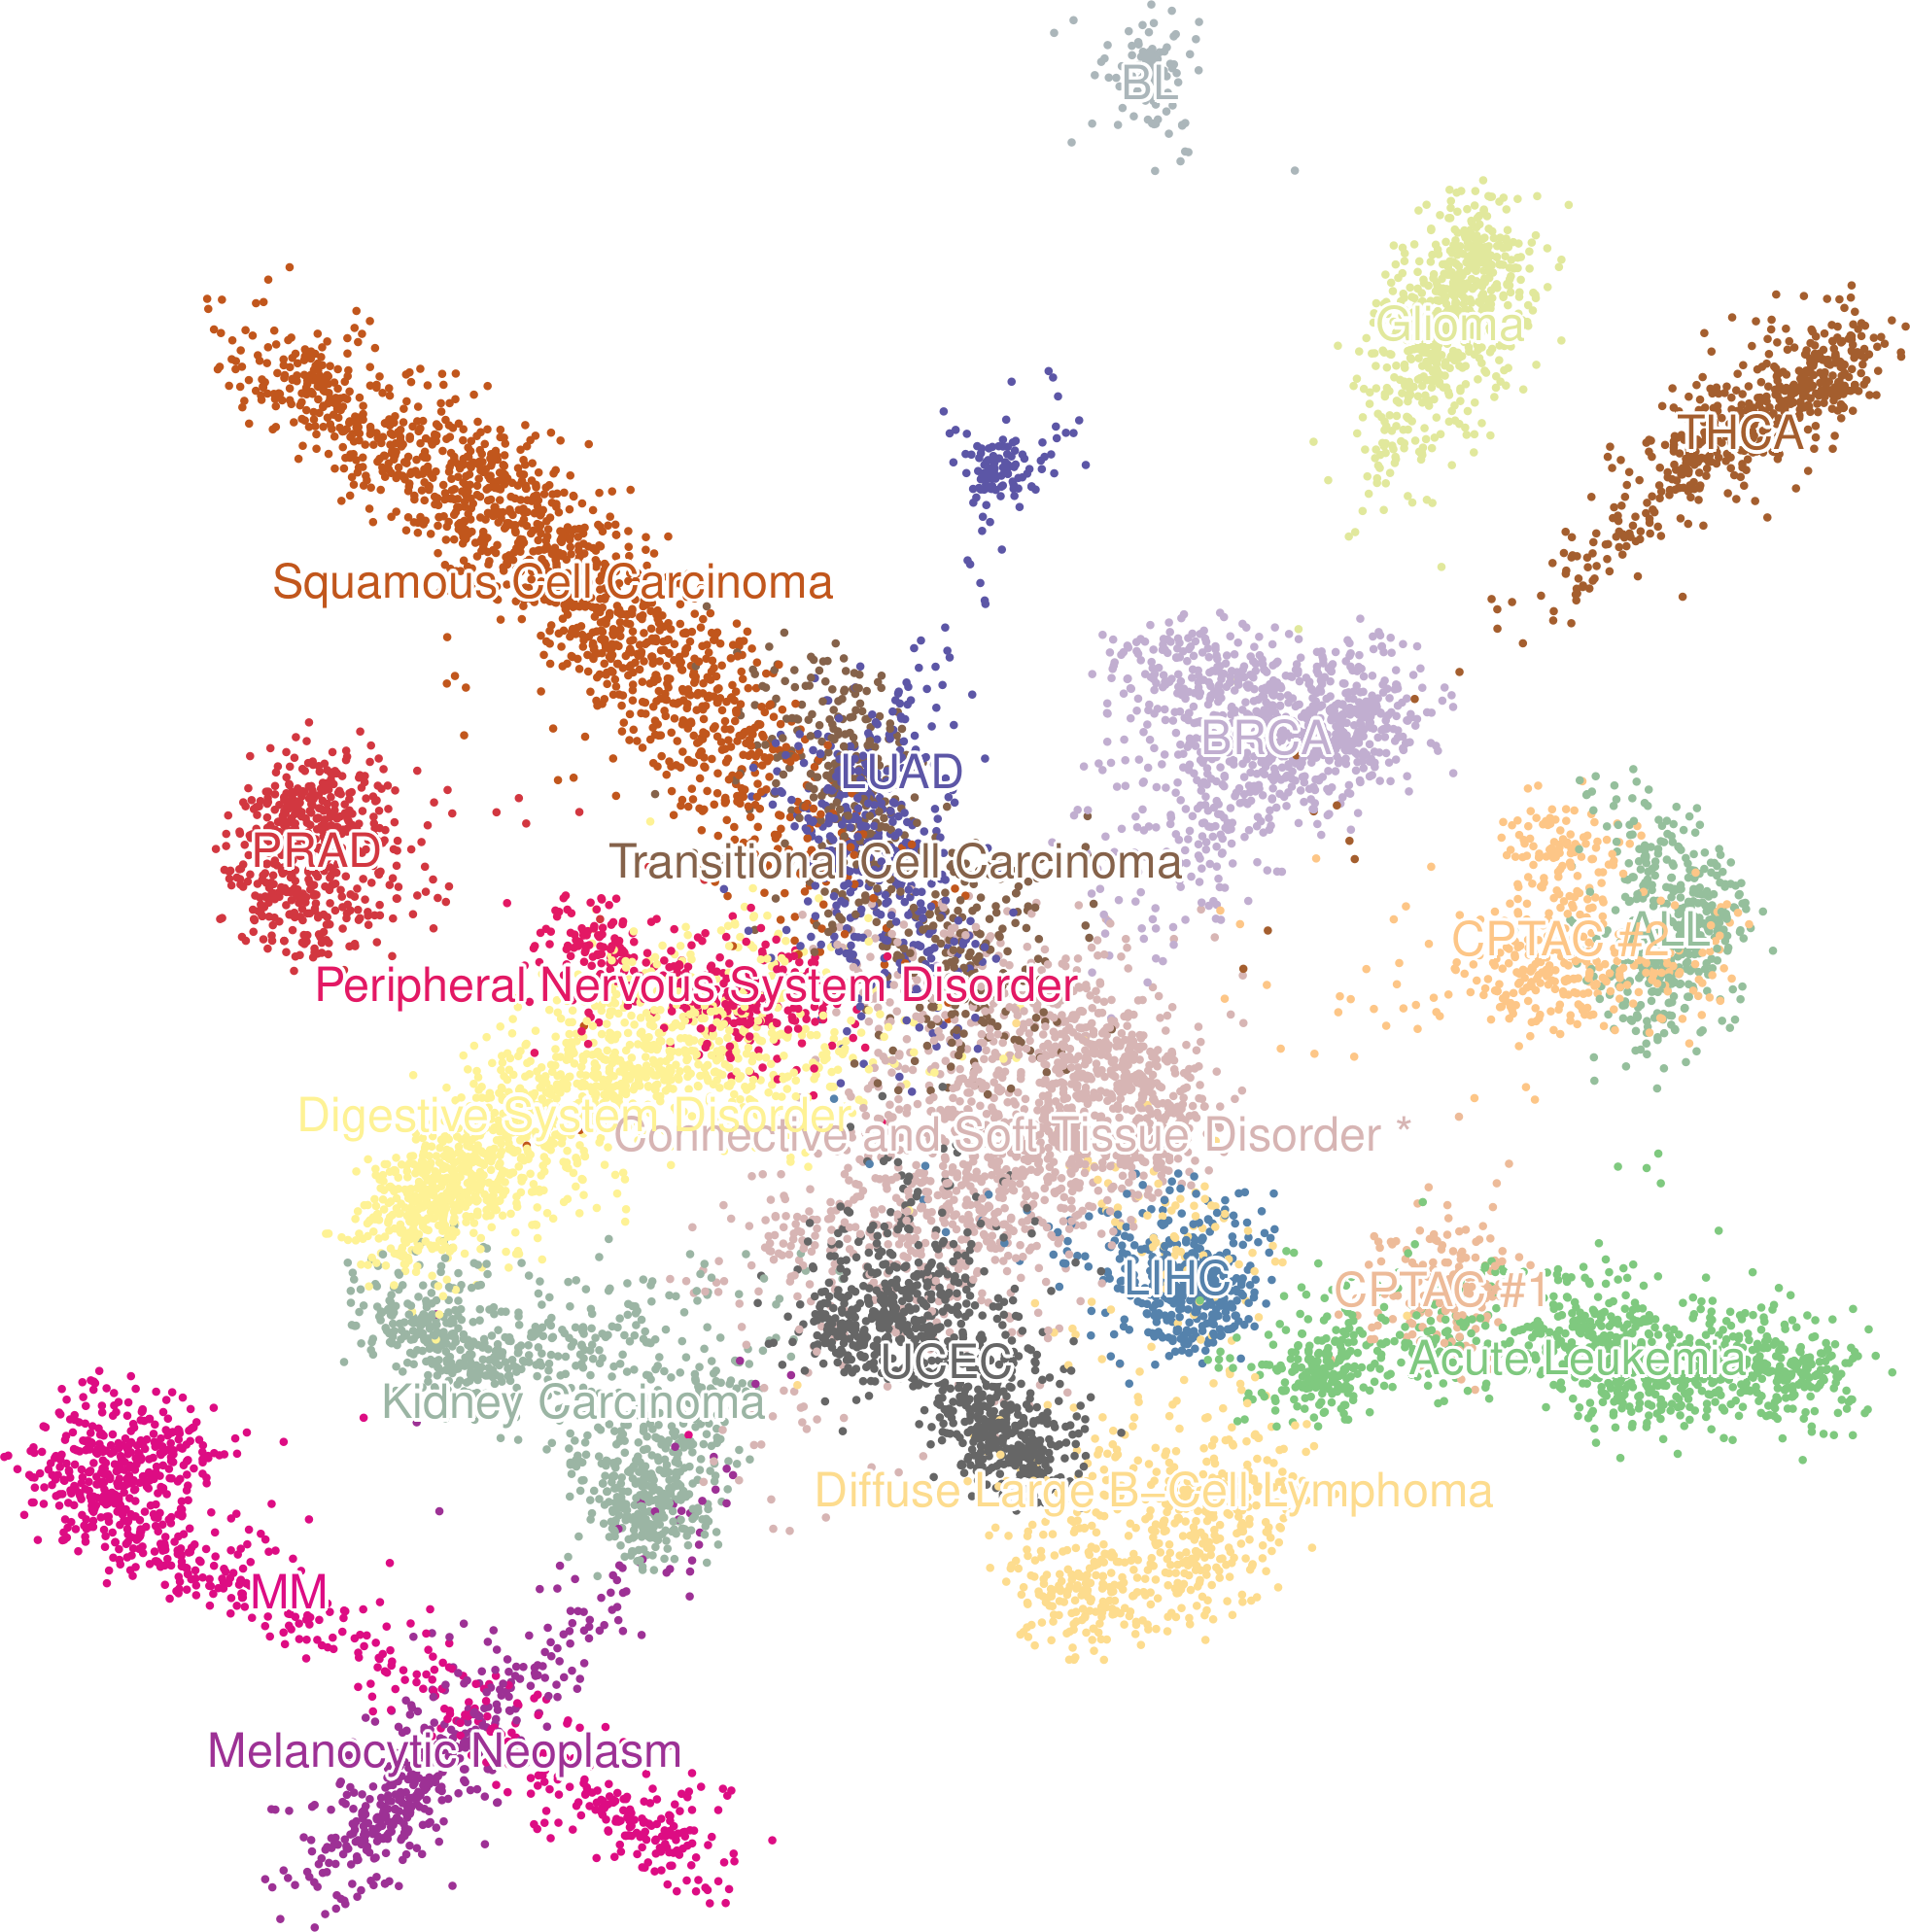
\includegraphics[width=.8\linewidth]{fig/tcga/plot_fr_cropped.png}\end{center}
	{\raggedright\textbf{B}}
	\begin{center}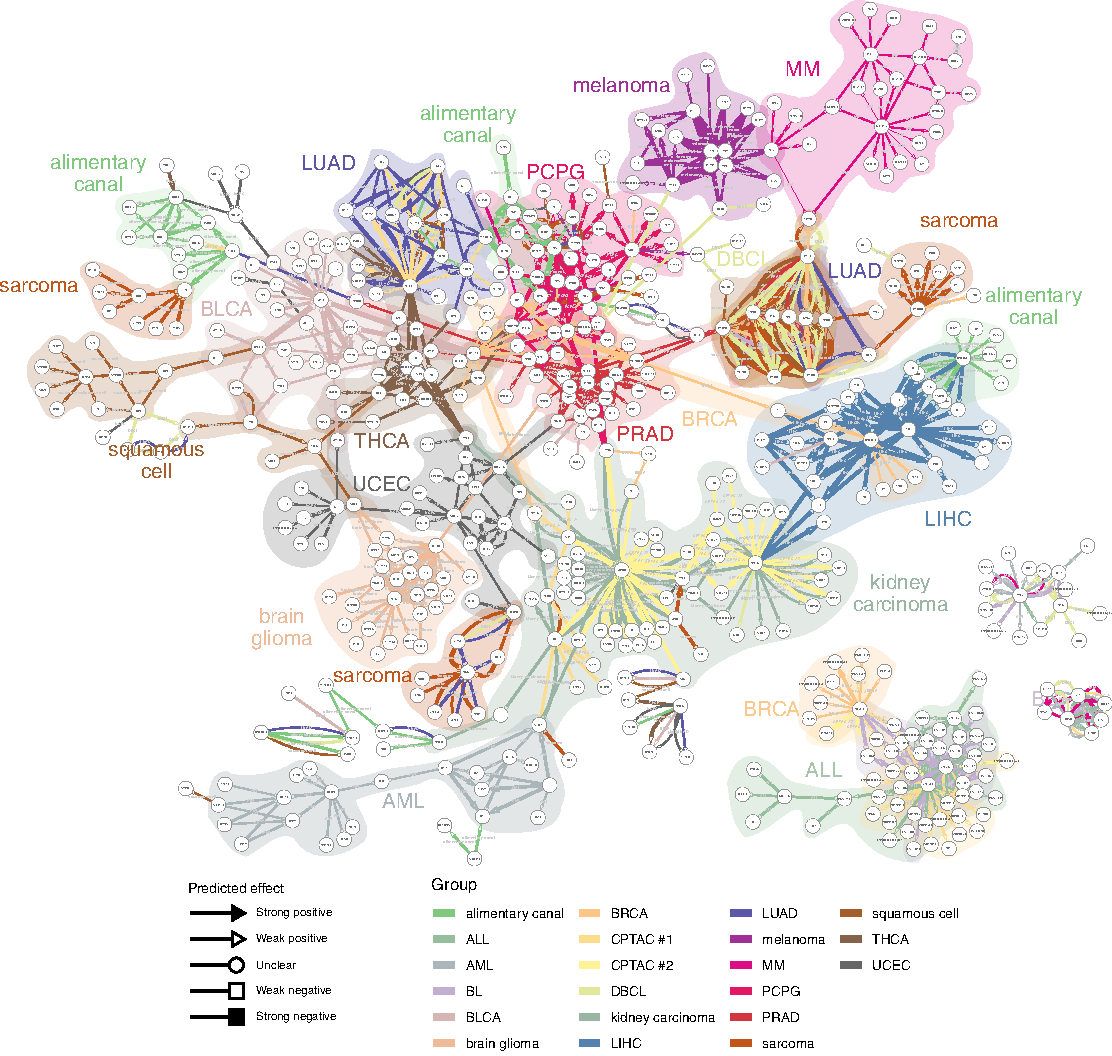
\includegraphics[width=.85\linewidth]{fig/tcga/grouped_interactions_2.pdf}\end{center}
	\caption{
		\textbf{14'963 case-wise GRNs of cancer bulk profiles from The Cancer Genome Atlas project.}
		\textbf{A:} The different profiles are visualised and clustered according to their regulomic similarities.
		\textbf{B:} Visualisation of the strongest interactions per cluster shows both pathways distinct to particular cancer entities as well as pathways common to multiple cancer entities.
	}
	\label{fig:tcga}
\end{figure}


\section{Discussion}

% going forward: functional validation; benchmark against in silico datasets; 
% can also use TI instead of clustering

\section{Methods}

\subsection{Inferring case-wise GRNs}
The task of inferring a static GRN (Figure~\ref{fig:simplify}A) can be reduced to a simpler problem, namely: for every target $T$, predict which of the potential regulators $R_i$ regulate $T$ (Figure~\ref{fig:simplify}B). This simplification allowed GENIE3\cite{huynh-thu_inferringregulatorynetworks_2010} to use Random Forest's\cite{breiman_randomforests_2001} feature importance scores for inferring GRNs. Namely, a Random Forest is trained to predict the expression of a target gene of interest from the expression of potential regulators. The resulting Random Forest inherently allows to extract a feature importance score by observing the effect of each regulator in making a good prediction for the target expression. As in GENIE3, the target expression is first scaled to normalise feature importance scores across different targets.

\begin{figure}[htb!]
	\centering
	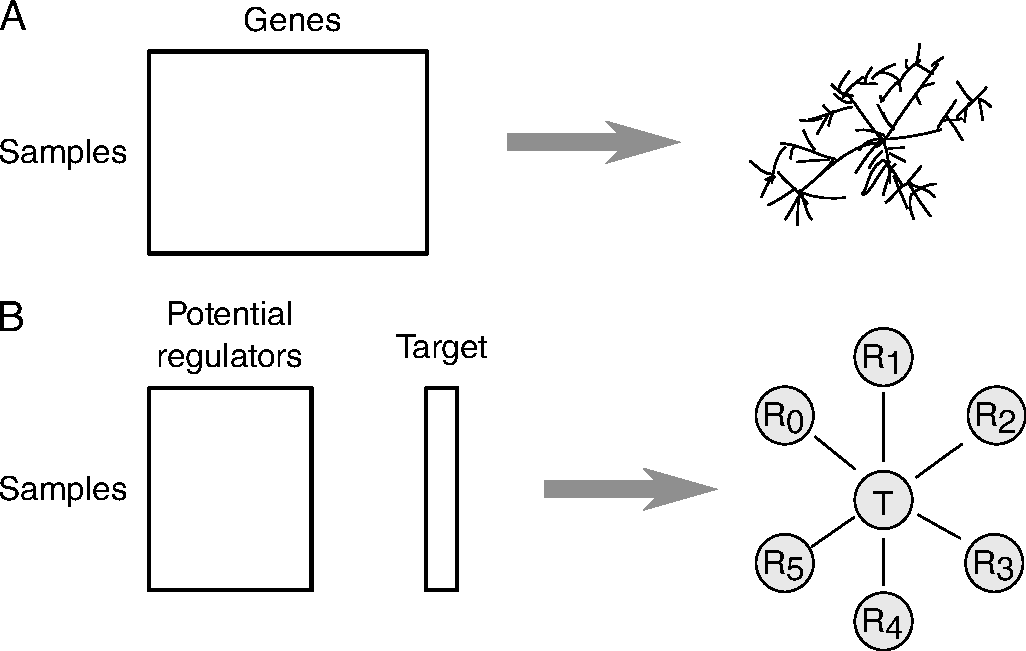
\includegraphics[width=.6\linewidth]{fig/methodology/simplify.pdf} 
	\caption{
		\textbf{A:} Inferring a gene regulatory network from an omics dataset can be reduced to a simpler problem. 
		\textbf{B:} Given the expression of a target of interest and a set of potential regulators, predict which regulators regulate the target gene.
	}
	\label{fig:simplify}
\end{figure}

We make the same simplification in order to build case-wise GRNs, also using Random Forests to compute the feature importance scores. A Random Forest consists of $K$ trees, each of which produces feature importance scores, and the feature importance scores of a forest is simply the mean feature importance scores of each of the trees. 

Computing the case-wise feature importances of a tree consists of the following 8 steps (Figure~\ref{fig:fimp}).
The 'randomness' of a Random Forest is due to only using a subset of the samples in the dataset in order to build a single decision tree. The samples are split into two groups, the 'in-bag' data and the 'out-of-bag' data (Figure~\ref{fig:fimp}A). A decision tree\cite{breiman_classificationregressiontrees_1984} is trained on the in-bag expression of the potential regulators in trying to predict the in-bag target gene expression (Figure~\ref{fig:fimp}B). The target expression of the out-of-bag samples is predicted using the decision tree (Figure~\ref{fig:fimp}C), and the squared error between the real and target expression is computed (Figure~\ref{fig:fimp}D). For each sample in the out-of-bag set, this vector represents how well the decision tree was able to predict the expression of the target gene.

The next few steps are repeated for every potential regulator $R_i$. Within the out-of-bag samples, the expression of $R_i$ is randomly shuffled. The target expression of the out-of-bag samples is again calculated (Figure~\ref{fig:fimp}F), as well as the squared error between the real target expression and the predicted expression is calculated (Figure~\ref{fig:fimp}G). The importance of regulator $R_i$ for an out-of-bag sample $S_j$ is defined as the increase in squared error between the predicted target expression and the real target expression, after perturbing the expression of $R_i$ (Figure~\ref{fig:fimp}H). 

Steps F-G are repeated for every potential regulator $R_i$. By aggregating all of the feature importance scores over all the samples, regulators and targets, we obtain an $M$-by-$N$-by-$P$ tensor\footnote{This is the origin of the name of the method, "\texttt{bred}".}. 

A moderately-sized dataset could contain $M=10'000$ samples, $N=2'000$ regulators, and $P=10'000$ target genes. Due to memory constrains, only interactions with an average importance value (across all samples) higher than a minimum threshold are retained.

\begin{figure}[htb!]
	\centering
	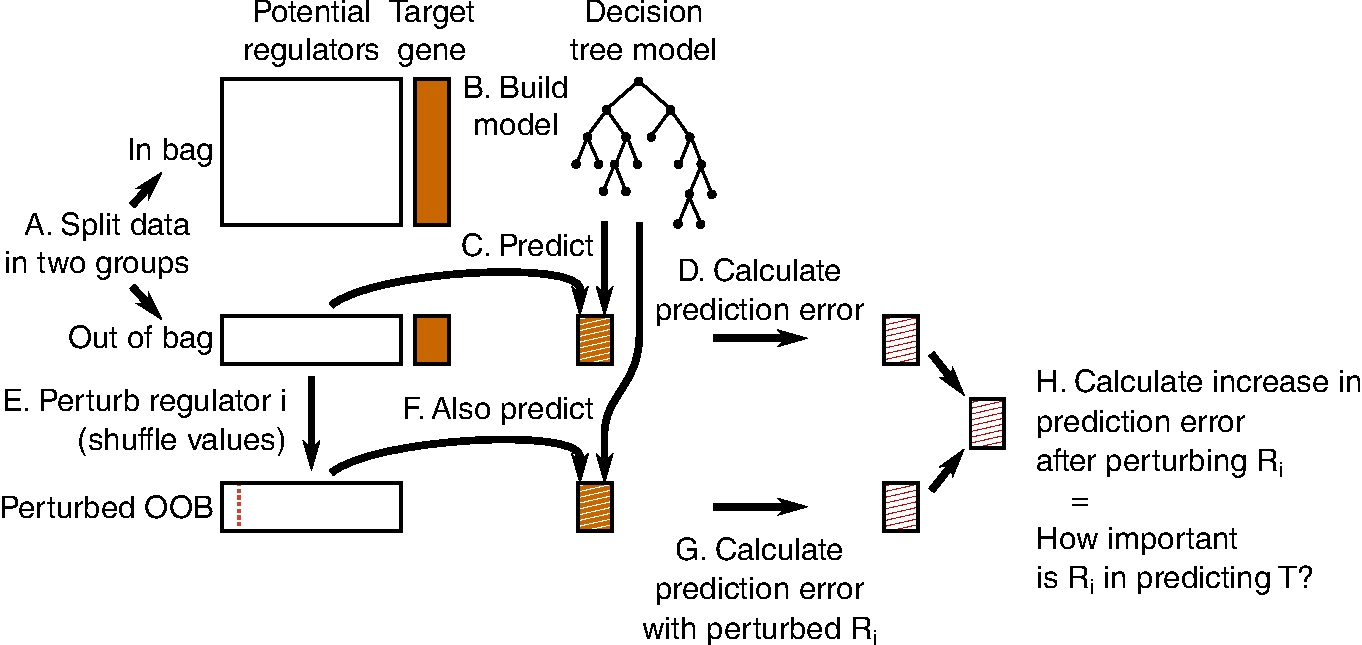
\includegraphics[width=.9\linewidth]{fig/methodology/fimp.pdf} 
	\caption{
		\textbf{Calculating the feature importance score for one decision tree and one target consists of 8 distinct steps.}
		\textbf{A:} Randomly split the data into two groups, the in-bag data and the out-of-bag data.
		\textbf{B:} The in-bag data is used to train a decision tree to try to predict the expression of the target gene from the expression values of the regulators.
		\textbf{C:} The decision tree is used to predict the gene expression of the target gene of the out-of-bag samples.
		\textbf{D:} Sample-specific squared error values are computed.
		\textbf{E:} Repeat steps E-H for every regulator $R_i$. Perturb the expression of regulator $R_i$ in the out-of-bag samples.
		\textbf{F:} Again predict the gene expression of the target gene with the perturbed expression values.
		\textbf{G:} Again compute the sample-specific squared error values.
		\textbf{H:} The difference between the prediction error on the perturbed dataset versus the prediction error on the unperturbed is the importance in $R_i$ in predicting $T$ 
	}
	\label{fig:fimp}
\end{figure}

To compute the case-wise GRNs, we implemented the abovementioned methodology in C++ in a modified version of the \texttt{ranger} R/C++ package\cite{wright_rangerfastimplementation_2017}.

\subsection{Predicting the effect of an interaction}
To predict the effect of a potential regulator $R_i$ on a target gene $T$ for a given tree, the Pearson correlation is calculated between the difference in regulator expression (before and after shuffling the values), and the difference in target expression prediction. 

\begin{align*}
  \text{effect}(R_i \rightarrow T) & = \text{cor}(x, y), \\
  \text{with } x & = \text{expr\_shuffled}[:,R_i] - \text{expr}[:,R_i], \\
  \text{and } y & = \text{predict}(\text{tree}, \text{expr\_shuffled}) - \text{predict}(\text{tree}, \text{expr}).
\end{align*}

The Pearson correlation between two variables $x$ and $y$ is usually defined as shown in Equation~\ref{eqn:pearson1}. Computing $r_{xy}$ for each (regulator, target) pairs, across all trees, would require storing large amounts of data.

\begin{equation}\label{eqn:pearson1}
	r_{xy} = \frac{\sum^n_{i=1} (x_i - \bar{x}) \times (y_i - \bar{y})}{\sqrt{\sum^n_{i=1}(x_i - \bar{x})^2}\times\sqrt{\sum^n_{i=1}(y_i - \bar{y})^2}}
\end{equation} 

However, by rearranging the formula, it can be defined as Equation~\ref{eqn:pearson2}.

\begin{equation}\label{eqn:pearson2}
r_{xy} = \frac{\sum(x_i \times y_i) - \sum x \times \sum y / n}{\sqrt{(\sum x_i^2 - (\sum x)^2 / n)} \times \sqrt{(\sum y_i^2 - (\sum y)^2 / n)}}
\end{equation}

For every regulator $R_i$ during a perturbation in a given tree, only 6 values need to be stored, namely $A = \sum x_i$, $B = \sum y_i$, $C = n$, $D = \sum{x_i \times y_i}$, $E = \sum{x_i \times x_i}$, and $F = \sum{y_i \times y_i}$.

For every (regulator, target) pair, these values are summed, and the $r_{xy}$ is calculated as shown in Equation~\ref{eqn:pearson3}.

\begin{equation}\label{eqn:pearson3}
r_{xy} = \frac{D - A \times B / C}{\sqrt{(E - A^2 / C)} \times \sqrt{(F - B^2 / C)}}
\end{equation}

The following cutoffs were used to determine the effect. 

\begin{itemize}
	\item Strong negative: $r_{xy} < -0.4$
  \item Weak negative: $-0.4 \leq r_{xy} < -0.2$
  \item Unclear: $-0.2 \leq r_{xy} \leq 0.2$
  \item Weak positive: $0.2 < r_{xy} \leq 0.4$
  \item Strong positive: $0.4 < r_{xy}$
\end{itemize} 

\subsection{Clustering of case-wise GRNs}
To perform downstream analysis on the cases, first a $k$-nearest neighbour ($k$NN) graph of the cases is computed.
In order for the $k$NN graph to better emphasise similarities in GRNs rather than absolute euclidean distances, we first reduce the dimensionality of the case-by-interaction matrix to case-by-20 matrix using Landmark Multi-Dimensional Scaling\cite{lee_landmarkmdsensemble_2009} with a Spearman rank distance metric.  

Next, KD-trees are used to calculate the $k$NN graph efficiently. The cases in the dataset are visualised and clusted using the Fruchterman-Reingold\cite{fruchterman_graphdrawingforcedirected_1991} and Louvain clustering\cite{blondel_fastunfoldingcommunities_2008}, respectively.

The following R packages provided implementations for each of these algorithms: lmds, RANN, igraph\cite{csardi_igraphsoftwarepackage_2006}.

\subsection{Visualising clustered GRNs}
After Louvain clustering, the interactions of the 50 interactions with highest mean importance per cluster are retained. These interactions are visualised in Cytoscape\cite{shannon_cytoscapesoftwareenvironment_2003}, in which nodes depict genes, edges depict predicted regulatory interactions, coloured according to which cluster they are predicted for. The shape of the arrow denotes the predicted effect of the regulatory interaction.

\subsection{Data from the Tabula Muris project}

\subsection{Data from The Canger Genome Atlas project}

\clearpage
\section{References}
\printbibliography[heading=none]
